\documentclass{ieeetmlcn}
\usepackage{cite}
\usepackage{amsmath,amssymb,amsfonts}
\usepackage{graphicx,color}
\usepackage{textcomp}
\usepackage{hyperref}
\usepackage{algorithm}
\usepackage{algpseudocode}
\usepackage{siunitx}
\usepackage{multirow}
\usepackage{float}
\usepackage{xcolor}
\usepackage[T1]{fontenc}
\usepackage{lmodern}
\usepackage{fix-cm}
\usepackage{tikz}
\newcommand{\Part}[2]{\Statex\textbf{Part #1:} #2\Statex}
\ifCLASSOPTIONcompsoc
    \usepackage[caption=false, font=normalsize, labelfont=sf, textfont=sf]{subfig}
\else
    \usepackage[caption=false, font=footnotesize]{subfig}
\fi

% Set Roman numerals for sections
\renewcommand{\thesection}{\Roman{section}}
\renewcommand{\thesubsection}{\thesection.\Alph{subsection}}
\renewcommand{\thesubsubsection}{\thesubsection.\arabic{subsubsection}}

\def\BibTeX{{\rm B\kern-.05em{\sc i\kern-.025em b}\kern-.08em
    T\kern-.1667em\lower.7ex\hbox{E}\kern-.125emX}}
\AtBeginDocument{\definecolor{tmlcncolor}{cmyk}{0.93,0.59,0.15,0.02}\definecolor{NavyBlue}{RGB}{0,86,125}}

\def\OJlogo{\vspace{-4pt}
\includegraphics[height=18pt]{format/new_logo.eps}}
\def\seclogo{\vspace{10pt}
\includegraphics[height=18pt]{format/new_logo.eps}}

\def\authorrefmark#1{\ensuremath{^{\textbf{#1}}}}

\begin{document}
\receiveddate{XX Month, XXXX}
\reviseddate{XX Month, XXXX}
\accepteddate{XX Month, XXXX}
\publisheddate{XX Month, XXXX}
\currentdate{XX Month, XXXX}
\doiinfo{TMLCN.2024.XXXXXXX}

\markboth{Transactions on Machine Learning in
Communications and Networking}{Berend J.D. Gort et al.}

\title{AERO: Adaptive Edge-Cloud Orchestration with a Sub-1K-Parameter Forecasting Model}

\author{Berend J.D. Gort\authorrefmark{1}, Godfrey M. Kibalya\authorrefmark{1}, and Angelos Antonopoulos\authorrefmark{1}}
\affil{\authorrefmark{1}Nearby Computing, Barcelona, Spain}
\corresp{Corresponding author: Berend J.D. Gort (email: berend.gort@nearbycomputing.com).}

% \authornote{This paragraph of the first footnote will contain support information, including sponsor and financial support acknowledgment. For example, ``This work was supported in part by the U.S. Department of Commerce under Grant 123456.''}

\begin{abstract}
Effective resource management in edge-cloud networks is crucial for meeting Quality of Service (QoS) requirements while minimizing operational costs. However, dynamic and fluctuating workloads pose significant challenges for accurate workload prediction and efficient resource allocation, particularly in resource-constrained edge environments. In this paper, we introduce \textbf{AERO} (Adaptive Edge-cloud Resource Orchestration), a novel lightweight forecasting model designed to address these challenges. AERO features an adaptive period detection mechanism that dynamically identifies dominant periodicities in multivariate workload data, allowing it to adjust to varying patterns and abrupt changes. With fewer than 1,000 parameters, AERO is highly suitable for deployment on edge devices with limited computational capacity. We formalize our approach through a comprehensive system model and extend an existing simulation framework with predictor modules to evaluate AERO's performance in realistic cloud-edge environments. Our extensive evaluations on real-world cloud workload datasets demonstrate that AERO achieves comparable prediction accuracy to complex state-of-the-art models with millions of parameters, while significantly reducing model size and computational overhead. Simulations show that AERO improves orchestration performance, achieving up to 13\% reduction in energy consumption and 67\% reduction in response times compared to reactive approaches. {\color{blue} Our live deployment experiments further validate these findings, demonstrating that AERO consistently delivers superior performance}. These results highlight AERO as an effective solution for improving resource management and reducing operational costs in dynamic cloud-edge environments.
\end{abstract}


\begin{IEEEkeywords}
Edge computing, cloud-edge orchestration, adaptive resource management, lightweight forecasting models, workload prediction, dynamic periodicity detection, resource-constrained environments, multivariate time series analysis
\end{IEEEkeywords}

%\IEEEspecialpapernotice{(Invited Paper)}

\maketitle

\section{INTRODUCTION}
\label{sec:introduction}

\IEEEPARstart{E}{dge} computing and cloud-native architectures are reshaping the computational landscape by bringing computational resources closer to end-users, enabling low-latency services \cite{10229034}. This shift enhances application performance but introduces challenges in optimizing resource utilization due to highly dynamic and fluctuating workloads in edge-cloud environments ~\cite{10229064, 8258257}. Efficient resource management is essential to meet Quality of Service (QoS) requirements while minimizing operational costs~\cite{8258257}.

Accurate workload prediction at the container level has become crucial for proactive orchestration and resource management in edge-cloud systems \cite{9068614}. The widespread adoption of microservice architectures has introduced new challenges, as applications are decomposed into numerous containers with intricate dependencies and resource consumption patterns \cite{10029931}. This architectural shift demands more granular predictions for effective container-specific elasticity operations. However, traditional prediction models struggle to capture these complex dynamics, as containerized microservices exhibit unpredictable demand fluctuations and frequent migrations across heterogeneous edge-cloud environments \cite{ouyang2023dynamic, benidis2022deep}.

The state-of-the-art in cloud workload prediction can be categorized into five main approaches \cite{kumar2018workload, tang2019large}. Evolutionary Learning methods integrate neural networks with evolutionary optimization techniques \cite{kumar2021self}. Deep Learning approaches form the predominant category, particularly focusing on temporal dependencies in cloud workloads \cite{zhang2018efficient, zhang2017resource}, though they face challenges with long-range predictions and rapid workload changes \cite{hochreiter1998vanishing}. Hybrid Learning combines multiple algorithms to overcome individual limitations \cite{kardani2020adrl, karim2021bhyprec}, while Ensemble Learning leverages multiple predictive models for improved accuracy \cite{singh2014ensemble, iqbal2019adaptive}. Finally, Quantum Learning has emerged as a promising direction for handling the complexity of modern cloud environments \cite{singh2021quantum}. However, most of these approaches rely on classical architectures like Recurrent Neural Networks (RNNs), while the machine learning literature has been rapidly evolving with newer architectures.

Recent machine learning advancements have introduced architectures like Graph Neural Networks (GNNs)~\cite{yi2024fouriergnn}, temporal Convolutional Neural Networks (CNNs)~\cite{donghao2024moderntcn}, and Transformer-based models~\cite{gort2024forecasting}. These models excel in capturing complex temporal patterns but are often computationally intensive due to their large number of parameters, making them unsuitable for resource-constrained edge devices \cite{meuser2024revisiting}. For example, models like WGAN~\cite{arbat2022wassersteinadversarialtransformercloud} and Pathformer~\cite{pathformer2024} contain millions of parameters, requiring substantial computational resources and energy consumption, which is impractical for many edge environments \cite{kong2022edge}.

To mitigate these limitations, lightweight Multi-Layer Perceptron (MLP) architectures ~\cite{ekambaram2023tsmixer} have been proposed. One of these models, SparseTSF ~\cite{sparseTSF} is based on sparse multilayer perceptrons (MLPs) and is designed for fast inference with minimal resource consumption, making it suitable for edge deployment. It achieves performance comparable to larger models while significantly reducing model size. However, SparseTSF assumes a fixed periodicity in workload data, limiting its adaptability in environments where workload patterns exhibit dynamic periodicities or abrupt changes.

Models assuming fixed periodicities may fail to capture sudden changes or multiple overlapping patterns ~\cite{sparseTSF}, leading to decreased prediction accuracy and suboptimal resource allocation. There is a critical need for lightweight models that can adaptively adjust to changing workload data to improve prediction accuracy and resource efficiency \cite{fan2019urbanedge}.

In this paper, we introduce \textbf{AERO} (\textbf{A}daptive \textbf{E}dge-cloud \textbf{R}esource \textbf{O}rchestration), a novel forecasting model designed to address the challenges of dynamic workload prediction in resource-constrained environments. AERO is a lightweight model with fewer than 1,000 parameters, making it suitable for deployment on edge devices with limited computational capacity. It incorporates an adaptive period detection mechanism that dynamically identifies dominant periods in workload data, allowing it to adjust to varying periodic patterns. This adaptability enhances prediction accuracy and resource allocation efficiency compared to models assuming fixed periodicities like SparseTSF.

To validate the effectiveness of AERO, we leveraged the \textbf{COSCO} (\textbf{C}oupled \textbf{S}imulation and \textbf{C}ontainer \textbf{O}rchestration) framework \cite{tuli2021cosco}, which provides a realistic emulation environment for service orchestration. COSCO accurately replicates real-world container behavior, including migration patterns, resource allocation, and system dynamics, enabling thorough evaluation of workload predictors without physical infrastructure costs. The framework's creators have extensively validated it against real fog computing environments, demonstrating high correlation between simulated and actual performance metrics \cite{tuli2021cosco}. As a novel contribution, we extend COSCO with a prediction interface.

Our key contributions are:
\begin{itemize}
    \item We propose AERO, a lightweight adaptive model for edge-cloud workload prediction that effectively handles workloads with multiple or changing periodicities in multivariate data.
    \item We demonstrate that AERO achieves comparable or better accuracy than state-of-the-art models while significantly reducing model size and computational overhead, suiting resource-constrained environments.
    \item We extend the COSCO simulation framework with a prediction interface.
    \item Through evaluations on real-world datasets and simulations, we demonstrate AERO's ability to improve resource allocation and reduce operational costs in edge-cloud environments.
\end{itemize}

{\color{blue}
The remainder of this paper is organized as follows: We first present the notation used throughout the paper in Table~\ref{tab:notation}.} Section~\ref{sec:related_works} reviews related work in time series forecasting. Section~\ref{sec:system_model} formulates the workload prediction problem. Section~\ref{sec:proposed_solution} details AERO's architecture and implementation. Section~\ref{sec:evaluation} evaluates AERO against existing models. Section~\ref{sec:simulations} presents simulation results, and Section~\ref{sec:conclusion} concludes with future directions.




% Table with notation summary
\begin{table}[!t]
\centering
\textcolor{blue}{
\caption{Notation Summary}
\label{tab:notation}
\begin{tabular}{|l|p{0.65in}|l|p{0.65in}|}
\hline
\textbf{Symbol} & \textbf{Desc.} & \textbf{Symbol} & \textbf{Desc.} \\
\hline
$\mathcal{H}$ & Nodes & $\mathcal{R}_t$ & Latency \\
$h_i$ & Node $i$ & $\mathcal{R}_t^n$ & Norm. time \\
$\mathcal{C}$ & Containers & $\mathcal{O}$ & Objective \\
$c_j$ & Container $j$ & $\alpha$ & $\mathcal{E}_t$ weight \\
$\mathcal{J}_c$ & Jobs in $c$ & $\Delta t$ & Time step \\
$j$ & Job ID & $\mathcal{J}_t^c$ & Done jobs \\
$a_j$ & Arrival time & $\Delta t_j$ & End time \\
$\mathbf{r}_j$ & Resources & $\mathbf{P}_t$ & State \\
$\rho_{h_i}$ & Power & $K$ & Kernel size \\
$\rho_{h_i}^m$ & Max power & $P$ & Period \\
$\mathcal{E}_t$ & Energy & $\hat{y}_{t+1}$ & Prediction \\
$L$ & Loss & $\theta$ & Parameters \\
$\mathbf{W}_t, \mathbf{W}_{t-\kappa+1:t}$ & Workload & $f$ & Features \\
$T$ & Time steps & $\Psi_{\boldsymbol{\phi}}$ & Predictor \\
$\kappa$ & Context & $\lambda$ & Horizon \\
\hline
\end{tabular}}
\end{table}
    
\section{RELATED WORK}
\label{sec:related_works}

Traditional cloud workload prediction approaches can be categorized into five main methodologies: Evolutionary Learning, Deep Learning, Hybrid Learning, Ensemble Learning, and Quantum Learning \cite{kumar2018workload, tang2019large}. However, these traditional methods have not kept pace with the rapid advancements in general-purpose time series forecasting architectures based on modern machine learning techniques.

Recent machine learning breakthroughs have introduced sophisticated model architectures that surpass these traditional methods in capturing complex temporal patterns \cite{acmtimeseriesreview2024}. These state-of-the-art architectures can be broadly categorized into several key areas.

RNNs~\cite{lai2018modelinglongshorttermtemporal, Jhin_2024, li2023learningpolarrepresentationextremeadaptive} have traditionally been pivotal in time series forecasting due to their ability to model sequential data. Recent works have proposed novel RNN architectures and training strategies to tackle challenges like long-term dependencies and interpretability. Some models integrate autoregressive recurrent networks with probabilistic forecasting, while others combine CNNs and RNNs for enhanced multivariate prediction \cite{li2024evogwp}.

CNNs~\cite{wang2023micn} have been adapted for time series forecasting by capturing local temporal patterns and hierarchical features. Research in this area focuses on specialized CNN architectures for time series data, multi-scale convolutional operations, and hybrid models combining CNNs with other techniques for improved performance. Approaches include deep architectures with residual links and fully-connected layers \cite{donghao2024moderntcn}. However, CNNs struggle to capture long-range dependencies in time series data due to their limited receptive field size \cite{wu2023timesnettemporal2dvariationmodeling}. They also lack the ability to model sequential dependencies inherent in time series, as they treat each input window independently.

For multivariate and spatio-temporal forecasting tasks, GNNs~\cite{yi2024fouriergnn, zhang2024irregular} model dependencies between different time series as graphs. Recent studies leverage both temporal and spatial information to improve forecasting accuracy. These methods often integrate GNNs with other deep learning techniques to capture complex dependencies. However, GNNs can be computationally expensive, especially for large-scale problems such as time series and complex dependency structures \cite{jin2024survey}.

Transformer architectures~\cite{wu2023timesnettemporal2dvariationmodeling} have achieved significant success in time series forecasting, particularly for long-term predictions \cite{vaswani2017attention}. Recent works aim to enhance the efficiency and effectiveness of Transformers by addressing temporal dependencies, capturing multi-scale patterns, and handling non-stationarity. Some models introduce methods to capture periodic patterns at different scales, while others focus on adapting to changing data distributions \cite{jia2024witran}. However, Transformer models typically have a large number of parameters, often in the millions, leading to high computational requirements \cite{liu2023nonstationary}.

An emerging trend involves utilizing LLMs~\cite{tang2023one, liu2023large} for time series forecasting, taking advantage of their rich representations and transfer learning capabilities. However, due to the billions of parameters in LLMs, these approaches often require substantial computational resources \cite{rasul2023forecasting}, making them less suitable for resource-constrained environments like edge-cloud systems, which is the focus of our work.\textbf{}

Due to their simplicity and computational efficiency, Multilayer Perceptron (MLP)-based models~\cite{zeng2023koopa, wu2023timemlp, liu2023fits} have gained attention. Recent research explores novel MLP architectures that can capture temporal dynamics without complex attention mechanisms. Strategies include leveraging mathematical theories and frequency domain representations to model temporal dependencies \cite{zhou2023patchTST}. However, MLP models such as SparseTSF~\cite{sparseTSF} assume a fixed periodicity in workload data, limiting their ability to adapt to changing patterns in workload data.

Our work addresses these limitations by proposing \textbf{AERO}, a lightweight adaptive edge-cloud workload forecasting model described in detail in Section~\ref{sec:proposed_solution}.

\section{SYSTEM MODEL}
\label{sec:system_model}

In this section, we formalize our cloud workload prediction framework through four key components: workload representation, workload prediction model, objective function, and edge-cloud network architecture. This formalization provides the mathematical foundation for comparing different architectural approaches.

\subsection{Workload Representation}

Let $\mathbf{W}_t = [W_t^{(1)},\, W_t^{(2)},\, \ldots,\, W_t^{(f)}]^\top \in \mathbb{R}^f$ represent the workload vector \cite{zhou2021informer} at discrete time step $t$, where $W_t^{(i)}$ denotes the $i$-th resource utilization feature (e.g., CPU, memory usage), $f$ is the number of features, and $t \in \{1, 2, \ldots, T\}$, with $T$ being the total number of time steps in the trace. The complete workload trace forms a multivariate time series:
\begin{equation}
\mathbf{W} = [\mathbf{W}_1,\, \mathbf{W}_2,\, \ldots,\, \mathbf{W}_T]^\top \in \mathbb{R}^{T \times f}.
\end{equation}

\subsection{Workload Prediction Model}

Our objective is to forecast future workload vectors based on historical observations. We define a prediction function $\Psi_{\boldsymbol{\phi}}: \mathbb{R}^{\kappa \times f} \rightarrow \mathbb{R}^{\lambda \times f}$, parameterized by $\boldsymbol{\phi} \in \mathbb{R}^p$, which represents the trainable parameters of the prediction model (e.g., weights and biases of a neural network). The function $\Psi_{\boldsymbol{\phi}}$ estimates the workload over a prediction horizon of length $\lambda$, where $\lambda \in \mathbb{N}$ and $\lambda \geq 1$:
\begin{equation}
\label{eq:forecast_workload}
\hat{\mathbf{W}}_{t+1:t+\lambda} = \Psi_{\boldsymbol{\phi}}\left( \mathbf{W}_{t-\kappa+1:t} \right),
\end{equation}
where $\kappa \in \mathbb{N}$, $\kappa \geq 1$, is the length of the historical context window, and $\mathbf{W}_{t-\kappa+1:t} \in \mathbb{R}^{\kappa \times f}$ denotes the sequence of past workload vectors used for prediction. The model architecture and training process are determined by hyperparameters $\boldsymbol{\theta} \in \Theta$, where $\Theta$ defines the search space of valid configurations \cite{hyperparamsdatasets}.

\subsection{Objective Function}

To learn the model parameters $\boldsymbol{\phi}$, we minimize a loss function that measures the prediction error between the forecasted workload $\hat{\mathbf{W}}_{t+1:t+\lambda}$ and the ground truth workload $\mathbf{W}_{t+1:t+\lambda}$ across all resource dimensions. We employ the Mean Squared Error (MSE) as our optimization objective, which penalizes larger prediction errors quadratically: 
\begin{equation}
\mathcal{L}(\boldsymbol{\phi}) = \frac{1}{\lambda} \sum_{i=1}^{\lambda} \left\| \mathbf{W}_{t+i} - \hat{\mathbf{W}}_{t+i} \right\|_2^2,
\end{equation}
where $\left\| \cdot \right\|_2$ denotes the Euclidean norm in $\mathbb{R}^f$ and $t \in \{1, 2, \ldots, T-\lambda\}$. This loss function computes the average squared distance between predicted and actual resource utilization vectors across the prediction horizon $\lambda$.

\subsection{Edge-cloud Network Architecture}

Our simulations utilize a heterogeneous edge-cloud network comprising edge devices, fog nodes, and cloud servers \cite{tuli2021cosco}. Let $\mathcal{H} = \{h_1, h_2, ..., h_N\}$ be the set of computational nodes. Each node $h_i \in \mathcal{H}$ possesses specific resource capacities defined as a vector $\mathbf{c}_i = [c_i^{\text{cpu}}, c_i^{\text{memory}}, c_i^{\text{disk}}, c_i^{\text{network}}]^\top$, where $c_i^{\text{cpu}}$ represents CPU capacity in MHz, $c_i^{\text{memory}}$ represents memory capacity in KB, $c_i^{\text{disk}}$ represents storage capacity with read/write speeds in KB/s, and $c_i^{\text{network}}$ represents network bandwidth in Gb/s.

Let $\mathcal{C}$ denote the set of containers, where each container is decomposed into a set of tasks $\mathcal{J}_c$ for container $c \in \mathcal{C}$. Each task $j \in \mathcal{J}_c$ has resource requirements $\mathbf{r}_j = [r_j^{\text{cpu}}, r_j^{\text{memory}}, r_j^{\text{disk}}, r_j^{\text{network}}]^\top$ and arrival time $a_j$, with measurements collected at regular intervals.

Container-level workload predictions inform task scheduling across nodes to optimize resource utilization and meet Quality of Service (QoS) requirements \cite{tuli2021cosco}. The scheduler employs these predictions to make proactive allocation decisions \cite{farhad2023ai}, aiming to minimize metrics such as energy consumption and Service Level Agreement (SLA) violations \cite{raith2024opportunistic}. This architecture supports evaluating container workload prediction models like AERO on orchestration performance, as detailed in Section~\ref{sec:simulations}.

\section{AERO ARCHITECTURE}
\label{sec:proposed_solution}

{\color{blue}
Edge-cloud environments pose unique challenges for resource orchestration due to their heterogeneity, resource constraints, and dynamic workload patterns. To address these challenges, we propose \textbf{AERO} (\textbf{A}daptive \textbf{E}dge-cloud \textbf{R}esource \textbf{O}rchestration), a lightweight forecasting model specifically tailored for adaptive workload prediction in edge-cloud settings. AERO is designed to operate efficiently on resource-constrained edge devices while maintaining the high prediction accuracy essential for effective scheduling decisions.
}

\subsection*{Model Overview}


The AERO model operates on the historical workload data $\mathbf{W}_{t-\kappa+1:t} \in \mathbb{R}^{\kappa \times f}$, where $\kappa$ is the context window length and $f$ is the number of features, as defined in Section~\ref{sec:system_model}. The model serves as the prediction function $\Psi_{\boldsymbol{\phi}}$ parameterized by $\boldsymbol{\phi} \in \mathbb{R}^p$, mapping historical workloads to future predictions over a horizon $\lambda$:

\begin{equation}
\label{eq:aero_prediction_function}
\hat{\mathbf{W}}_{t+1:t+\lambda} = \Psi_{\boldsymbol{\phi}}\left( \mathbf{W}_{t-\kappa+1:t} \right).
\end{equation}

The AERO architecture consists of three main components:
\begin{enumerate}[A.]
    \item \texttt{Adaptive Period Detection Module}: Identifies and adapts to the dominant period $\tau$ within the historical workload data by analyzing temporal patterns.

    \item \texttt{Adaptive Forecasting Module}: Adjusts the detected period and performs forecasting using the SparseTSF model~\cite{sparseTSF}. This module handles the core prediction task, leveraging the strengths of SparseTSF for efficient time series forecasting.

    \item \texttt{Adaptive Layer Caching}: Maintains a cache of neural network layers optimized for different periodicities. When similar workload patterns recur, the model reuses these cached layers instead of recomputing them, significantly reducing computational overhead.
\end{enumerate}

{\color{blue}
By integrating these components, AERO provides a scalable solution deployed on distributed edge nodes. Its lightweight design minimizes computational complexity and memory footprint, making it suitable for resource-constrained devices. With few parameters, the model enables efficient retraining and online updates directly on edge devices, allowing inexpensive adaptation to dynamic workloads. This localized approach reduces communication overhead, as each edge node updates its model independently without transmitting large data. Overall, AERO's adaptability and efficiency ensure consistent, reliable performance across heterogeneous environments.

In the following sections, we delve into the detailed workings of each component of the AERO model. The algorithmic workflow of AERO is presented in Algorithm 1.
}

\subsection{Adaptive Period Detection Module}
\label{sec:adaptive_period_detection}

{\color{blue}
Detecting the dominant period $\tau$ is critical, as it directly determines the model's configuration for optimal performance. The parameter $\tau$ dictates how the model segments and processes the time series data, influencing its ability to accurately capture and leverage periodic patterns. By precisely identifying $\tau$, we ensure that the model aligns with the inherent periodicity of the data, effectively separating periodic components from trends and increasing forecasting accuracy.
}

The \texttt{Adaptive Period Detection Module} aims to identify the dominant period $\tau$ within the historical workload data sequence $\mathbf{W}_{t-\kappa+1:t}$. First, we compute the average across the feature dimension to obtain a univariate time series $\bar{\mathbf{W}}_{t-\kappa+1:t} \in \mathbb{R}^\kappa$:

\begin{equation}
\label{eq:feature_avg}
\bar{\mathbf{W}}_{t-\kappa+1:t} = \frac{1}{f} \sum_{i=1}^{f} \mathbf{W}_{t-\kappa+1:t}^{(i)},
\end{equation}
where $\mathbf{W}_{t-\kappa+1:t}^{(i)}$ denotes the $i$-th feature of the workload data sequence $\mathbf{W}_{t-\kappa+1:t}$.

Next, we subtract the mean to focus on the periodic components, yielding the mean-centered series $\tilde{\mathbf{W}}_{t-\kappa+1:t}$:

\begin{equation}
\label{eq:mean_removal}
\tilde{\mathbf{W}}_{t-\kappa+1:t} = \bar{\mathbf{W}}_{t-\kappa+1:t} - \boldsymbol{\mu}_{t-\kappa+1:t},
\end{equation}
where $\boldsymbol{\mu}_{t-\kappa+1:t} = \frac{1}{\kappa} \sum_{s=t-\kappa+1}^{t} \bar{\mathbf{W}}_s$ is the mean of the averaged workload sequence.

{\color{blue}
To efficiently identify the dominant period $\tau$, we begin by computing the autocorrelation function (ACF) of the mean-centered workload sequence $\tilde{\mathbf{W}}_{t-\kappa+1:t}$. The autocorrelation function measures the similarity between the time series and its lagged versions, which is essential for detecting repeating patterns and periodicities in the data.

The autocorrelation function is computed using convolution~\cite{zhang2020autocorrelation}:
\begin{equation}
\label{eq:acf}
\text{ACF}(\ell) = \frac{(\tilde{\mathbf{W}}_{t-\kappa+1:t} \ast \tilde{\mathbf{W}}^{\text{rev}}_{t-\kappa+1:t})[\ell]}{\text{ACF}(0) + \epsilon}, \quad \epsilon = 10^{-8},
\end{equation}
where $\ell \in \{0, 1, 2, \ldots, \kappa-1\}$ is the lag or time shift, $\tilde{\mathbf{W}}^{\text{rev}}_{t-\kappa+1:t}$ is the time-reversed version of $\tilde{\mathbf{W}}_{t-\kappa+1:t}$, $\ast$ denotes the convolution operation, and $\text{ACF}(0)$ is the variance of $\tilde{\mathbf{W}}_{t-\kappa+1:t}$. Computing the ACF via convolution allows us to leverage the Fast Fourier Transform (FFT~\cite{nussbaumer1982fast}), reducing the computational complexity from $\mathcal{O}(n^2)$ to $\mathcal{O}(n \log n)$ for large $n$. This efficiency is important for real-time processing on resource-constrained edge devices, enabling rapid analysis of temporal dependencies without significant computational overhead.

After obtaining the ACF, we identify peaks, which are points where the autocorrelation is higher than its immediate neighbors:
\begin{equation}
\label{eq:peak_detection}
\text{peaks} = \left\{ \ell \,\middle|\, \text{ACF}(\ell-1) < \text{ACF}(\ell) > \text{ACF}(\ell+1) \right\}.
\end{equation}
These peaks correspond to potential periods in the data.
}

Candidate periods $\mathcal{K}$ are selected from the peaks within the desired range $[\tau_{\min}, \tau_{\max}]$ (model hyperparameters):
\begin{equation}
\label{eq:candidate_periods}
\mathcal{K} = \left\{ \ell \in \text{peaks} \,\middle|\, \tau_{\min} \leq \ell \leq \tau_{\max} \right\}.
\end{equation}

Finally, the dominant period $\tau$ is assigned based on the candidate periods:
\begin{equation}
\label{eq:period_assignment}
\tau = \begin{cases}
    \left\lfloor \dfrac{\tau_{\max}}{2} \right\rfloor, & \text{if } \mathcal{K} = \emptyset, \\[2ex]
    \displaystyle\arg\max_{\ell \in \mathcal{K}} \text{ACF}(\ell), & \text{otherwise}.
\end{cases}
\end{equation}
{\color{blue}
When no candidate periods are found, we default to $\tau = \left\lfloor \dfrac{\tau_{\max}}{2} \right\rfloor$. This choice ensures at least two complete segments within the maximum period range (a hyperparameter), providing the minimum basis for temporal comparison in the absence of periodic patterns. A larger $\tau$ would yield insufficient segments for comparison, while a smaller $\tau$ risks over-segmentation. This balanced approach maintains the model's ability to capture potential temporal relationships even without explicit periodicity.}

\subsection{Adaptive Forecasting Module}
\label{sec:adaptive_forecasting}

After detecting the dominant period $\tau$ from the historical data, the \texttt{Adaptive Forecasting Module} adjusts this period to ensure compatibility with the model architecture and proceeds to predict future workloads $\hat{\mathbf{W}}_{t+1:t+\lambda} \in \mathbb{R}^{\lambda \times f}$, where $\lambda$ is the prediction horizon.

We first clamp the detected period $\tau$ to a valid range and make it even to satisfy the model's requirements:

\begin{equation}
\label{eq:tau_clamp}
\tau^\prime = \text{clamp}\left( \tau,\, 2,\, \left\lfloor \dfrac{\kappa}{2} \right\rfloor \right), \quad \tau^\prime = \tau^\prime + (\tau^\prime \bmod 2).
\end{equation}

Clamping $\tau$ ensures that the period is within a feasible range based on the context window length $\kappa$, and making it even simplifies subsequent segmentation and reshaping operations.

Next, we adjust the clamped period $\tau^\prime$ to the closest common divisor of $\kappa$ and $\lambda$:

\begin{equation}
\label{eq:tau_adjust}
\tau^{\ast} = \arg\min_{d \in D} \left| d - \tau^\prime \right|,
\end{equation}
where $D$ is the set of common divisors of $\kappa$ and $\lambda$. Adjusting $\tau^\prime$ to $\tau^{\ast}$ ensures that both the input sequence and the prediction horizon can be evenly divided into segments of length $\tau^{\ast}$, facilitating efficient downsampling and upsampling in the model.

After this point, the forecasting process follows the standard SparseTSF model~\cite{sparseTSF}. For completeness, we outline their forecasting process below.

First, the input data is normalized by subtracting the mean vector:

\begin{equation}
\label{eq:normalization}
\tilde{\mathbf{W}}_{t-\kappa+1:t} = \mathbf{W}_{t-\kappa+1:t} - \mathbf{1} \boldsymbol{\mu}_{t-\kappa+1:t}^\top \in \mathbb{R}^{\kappa \times f},
\end{equation}
where $\mathbf{1} \in \mathbb{R}^{\kappa}$ is a column vector of ones, and $\boldsymbol{\mu}_{t-\kappa+1:t} = \frac{1}{\kappa} \sum_{s=t-\kappa+1}^{t} \mathbf{W}_{s} \in \mathbb{R}^{1 \times f}$.

The normalized data is then transposed to align dimensions for convolution:

\begin{equation}
\label{eq:permutation}
\tilde{\mathbf{W}} = \tilde{\mathbf{W}}^\top \in \mathbb{R}^{f \times \kappa}.
\end{equation}

A one-dimensional convolution is applied with residual connection:

\begin{equation}
\label{eq:convolution}
\mathbf{Z} = \text{Conv1D}\left( \tilde{\mathbf{W}}; k,\, p \right) + \tilde{\mathbf{W}} \in \mathbb{R}^{f \times \kappa},
\end{equation}
where the kernel size $k = 1 + 2(\tau^{\ast}/2)$ and padding $p = \tau^{\ast}/2$.

The data is then downsampled through reshaping:

\begin{equation}
\label{eq:downsampling}
\mathbf{Z} = \text{reshape}\left( \mathbf{Z},\, \left[ f \cdot \tau^{\ast},\, n_x \right] \right) \in \mathbb{R}^{(f \cdot \tau^{\ast}) \times n_x},
\end{equation}
where $n_x = \kappa / \tau^{\ast}$ represents the number of segments in the input sequence.

A linear transformation maps the downsampled segments to prediction segments:

\begin{equation}
\label{eq:linear_mapping}
\mathbf{Y} = \text{Linear}\left( \mathbf{Z} \right) \in \mathbb{R}^{(f \cdot \tau^{\ast}) \times n_y},
\end{equation}
where $n_y = \lambda / \tau^{\ast}$ represents the number of segments in the prediction sequence.

The predictions are then upsampled through reshaping:

\begin{equation}
\label{eq:upsampling}
\mathbf{Y} = \text{reshape}\left( \mathbf{Y},\, \left[ f,\, \lambda \right] \right) \in \mathbb{R}^{f \times \lambda}.
\end{equation}

Finally, the predictions are denormalized:

\begin{equation}
\label{eq:denormalization}
\hat{\mathbf{W}}_{t+1:t+\lambda} = \mathbf{Y}^\top + \mathbf{1} \boldsymbol{\mu}^\top \in \mathbb{R}^{\lambda \times f}.
\end{equation}

This sequence of operations efficiently processes the time series data while maintaining its periodic structure. In our implementation, we leverage this architecture with our adaptively detected period $\tau^{\ast}$.


\subsection{Adaptive Layer Caching Mechanism}
\label{sec:adaptive_layer_caching}

{\color{blue}
In dynamic edge-cloud environments, workloads exhibit varying periodicities. To efficiently adapt without significant overhead, we introduce an \texttt{Adaptive Layer Caching Mechanism} in the AERO model. For each feasible period $\tau$ within a practical range $[\tau_{\min}, \tau_{\max}]$, we cache pre-initialized neural network layers configured specifically for that $\tau$. These layers include convolutional layers with kernel size $k = 1 + 2\left( \frac{\tau}{2} \right)$ and padding $\frac{\tau}{2}$, and linear layers mapping input segments of size $n_x = \kappa / \tau$ to output segments of size $n_y = \lambda / \tau$.

When the dominant period $\tau$ is detected (as per Section~\ref{sec:adaptive_period_detection}), it may not exactly match a cached period. In such cases, we adjust $\tau$ to the nearest cached value using Eq.~\eqref{eq:tau_adjust}. This adjustment is acceptable because small variations in period length often correspond to similar temporal patterns in the workload data. The model's convolutional and linear layers are designed to be robust to minor discrepancies in $\tau$, effectively capturing temporal dependencies even when the period is slightly adjusted. By using the nearest cached period, we ensure that only valid, pre-initialized layers are utilized, preventing mismatches and maintaining model integrity without significant loss in prediction accuracy.
}

\begin{algorithm}
\caption{AERO Model Implementation}
\label{alg:aero_impl}
\small
\begin{algorithmic}[1]
\Require
    \Statex \hspace{-1em}\textbf{Input:}
    \State Historical workload data $\mathbf{W}_{t-\kappa+1:t} \in \mathbb{R}^{\kappa \times f}$
    \State Prediction horizon $\lambda$
    \State Context window length $\kappa$
    \State Period range $[\tau_{\min}, \tau_{\max}]$
\Ensure
    \Statex \hspace{-1em}\textbf{Output:}
    \State Forecasted workloads $\hat{\mathbf{W}}_{t+1:t+\lambda} \in \mathbb{R}^{\lambda \times f}$
\Statex
\Part{1}{Adaptive Period Detection}
    \State Compute $\bar{\mathbf{W}}_{t-\kappa+1:t}$ using Eq.~\eqref{eq:feature_avg}
    \State Subtract mean to get $\tilde{\mathbf{W}}_{t-\kappa+1:t}$ \hfill {\small(Eq.~\eqref{eq:mean_removal})}
    \State Compute $\text{ACF}(\ell)$ using convolution \hfill {\small(Eq.~\eqref{eq:acf})}
    \State Detect peaks and select $\tau$ \hfill {\small(Eqs.~\eqref{eq:peak_detection}--\eqref{eq:period_assignment})}
\Statex
\Part{2}{Period Adjustment}
    \State Adjust $\tau$ to $\tau^{\ast}$ \hfill {\small(Eqs.~\eqref{eq:tau_clamp} and \eqref{eq:tau_adjust})}
\Statex
\Part{3}{Adaptive Forecasting (SparseTSF)}
    \State Normalize data \hfill {\small(Eq.~\eqref{eq:normalization})}
    \State Reshape for convolution \hfill {\small(Eq.~\eqref{eq:permutation})}
    \State Apply convolution with residual connection \hfill {\small(Eq.~\eqref{eq:convolution})}
    \State Downsample data \hfill {\small(Eq.~\eqref{eq:downsampling})}
    \State Perform linear mapping \hfill {\small(Eq.~\eqref{eq:linear_mapping})}
    \State Upsample predictions \hfill {\small(Eq.~\eqref{eq:upsampling})}
    \State Denormalize outputs \hfill {\small(Eq.~\eqref{eq:denormalization})}
\Statex
\Part{4}{Output}
    \State \Return $\hat{\mathbf{W}}_{t+1:t+\lambda}$
\end{algorithmic}
\end{algorithm}

\section{EVALUATION}

In this section, we present the evaluation of our proposed AERO model through two comprehensive scenarios. First, we conduct a performance evaluation of machine learning models, where we benchmark AERO against five state-of-the-art approaches using metrics including prediction accuracy, computational efficiency, and model complexity. Second, we perform an orchestration performance evaluation to assess how these prediction models impact fog computing environments, analyzing metrics such as energy consumption, response time, resource utilization, and SLA violations.

\subsection{Performance Evaluation of Machine Learning Models}
\label{sec:evaluation}

In this section, we conduct a comprehensive machine learning evaluation to assess model performance across multiple dimensions: prediction accuracy, computational efficiency, and adaptability to dynamic workload patterns.

\subsubsection{Dataset}

We use the Alibaba 2022 microservices trace dataset~\cite{luo2022Prediction}, focusing on pod \texttt{MS\_11349}. The dataset provides $T = 18,\!720$ samples collected at 1-minute intervals over 13 days. Each workload vector $\mathbf{W}_t \in \mathbb{R}^{f}$ consists of $f = 2$ features: normalized CPU utilization ($W_t^{(1)}$) and memory utilization ($W_t^{(2)}$), aligning with the workload representation in Section~\ref{sec:system_model}. This forms a workload trace $\mathbf{W} \in \mathbb{R}^{T \times f}$ exhibiting both deterministic trends $\boldsymbol{\mu}_t$ (e.g., daily patterns) and stochastic fluctuations $\boldsymbol{\epsilon}_t$ (e.g., demand spikes), making it ideal for evaluating prediction models with different historical context windows $\kappa$ and forecast horizons $\lambda$.

\subsubsection{Benchmarks}

We compare AERO with five state-of-the-art models, each representing a distinct architecture:

\begin{itemize}
    \item \textbf{FourierGNN}~\cite{yi2024fouriergnn} combines Graph Neural Networks (GNNs) with Fourier transforms to capture complex spatio-temporal dependencies.
    \item \textbf{ModernTCN}~\cite{donghao2024moderntcn} employs Temporal Convolutional Networks (TCNs) with advanced dilation to model long-range dependencies efficiently.
    \item \textbf{WGAN}~\cite{arbat2022wassersteinadversarialtransformercloud} is a transformer-based model utilizing a generative adversarial approach, representing the state-of-the-art in cloud-native workload prediction.
    \item \textbf{Pathformer}~\cite{pathformer2024}, designed by Alibaba Group, optimizes the Transformer architecture with efficient attention mechanisms.
    {\color{blue}
    \item \textbf{DLinear}~\cite{DLinear} is a lightweight model that decomposes time series into trend and seasonal components using moving averages, processes each with separate linear layers, and combines them for prediction.}
    \item \textbf{SparseTSF}~\cite{sparseTSF} is a lightweight framework based on sparse MLPs, designed for fast inference and minimal resource consumption.
\end{itemize}

\subsubsection{Experimental Settings}

{\color{blue}
All experiments were conducted on a server with NVIDIA A100 GPU (40 GB), 30 CPU cores, 200 GiB RAM, running Ubuntu 20.04.2 LTS. Models were implemented in PyTorch, and MLFlow tracked all experiments. To ensure fair comparisons, we standardized the experimental setup. Our hyperparameter tuning method used Bayesian optimization (BoTorch \cite{balandat2020botorch}, GPyTorch \cite{gardner2018gpytorch}) with ranges from original authors (Table \ref{tab:hyperparameter_ranges}). Each model had 20 random hyperparameter evaluations, followed by 30 optimization runs (totaling 50 training runs per model), optimizing for validation loss. All parameters were logged to MLFlow \cite{MLFlow}.

Per individual training run, models trained up to 100 epochs with early stopping (patience 10), optimizing validation loss. We used identical learning rate schedulers. Data were identically partitioned, and input was uniformly normalized and rescaled. Preprocessing steps ensured identical inputs. We used the same random seed for reproducibility.

By aligning hyperparameter tuning, training protocols, computational resources, data handling, and evaluation metrics, we minimized biases, ensuring fair comparisons and strengthening our conclusions.
}

We assess model performance using Mean Absolute Error (MAE) and Root Mean Square Error (RMSE), the two most commonly used metrics in time-series forecasting \cite{acmtimeseriesreview2024}:

\begin{equation}
\label{eq:mae}
\text{MAE} = \frac{1}{\lambda} \sum_{i=1}^{\lambda} \left\| \mathbf{W}_{t+i} - \hat{\mathbf{W}}_{t+i} \right\|_1,
\end{equation}

\begin{equation}
\label{eq:rmse}
\text{RMSE} = \sqrt{ \frac{1}{\lambda} \sum_{i=1}^{\lambda} \left\| \mathbf{W}_{t+i} - \hat{\mathbf{W}}_{t+i} \right\|_2^2 },
\end{equation}

where $\left\| \cdot \right\|_1$ and $\left\| \cdot \right\|_2$ denote the $\ell_1$ and Euclidean norms, respectively. In addition to prediction accuracy, we evaluate practical deployment considerations including inference time, convergence speed, parameter count, and memory usage.

\begin{table*}[t]
\centering
\caption{Hyperparameter Ranges for Bayesian Optimization Per Model}
\label{tab:hyperparameter_ranges}
\resizebox{\textwidth}{!}{%
\begin{tabular}{llccccccc}
\hline
\textbf{Hyperparameter} & \textbf{Symbol} & \textbf{FourierGNN} & \textbf{WGAN-GP} & \textbf{ModernTCN} & \textbf{Pathformer} & \textbf{SparseTSF} & \textcolor{blue}{\textbf{DLinear}} & \textbf{AERO (ours)} \\
\hline
Sequence length & $L_s$ & (48, 256) & (12, 48) & (48, 336) & (48, 96) & (48, 128) & \textcolor{blue}{(60, 140)} & (48, 128) \\
Prediction length & $L_p$ & (12, 96) & (1, 24) & (12, 96) & (12, 96) & (12, 24) & \textcolor{blue}{(12, 30)} & (12, 24) \\
Batch size & $B$ & (16, 128) & (16, 128) & (32, 512) & (128, 512) & (128, 512) & \textcolor{blue}{(100, 500)} & (128, 512) \\
Model dimension & $d_m$ & - & (16, 128) & (32, 512) & (4, 16) & (64, 512) & \textcolor{blue}{(32, 256)} & (64, 512) \\
Number of heads & $N_h$ & - & (2, 8) & (1, 8) & - & - & \textcolor{blue}{-} & - \\
Encoder layers & $L_e$ & - & (1, 4) & (1, 4) & (1, 3) & (1, 3) & \textcolor{blue}{(1, 2)} & (1, 3) \\
Decoder layers & $L_d$ & - & (1, 4) & - & - & - & \textcolor{blue}{-} & - \\
Dropout & $p_d$ & (0.0, 0.5) & (0.0, 0.5) & (0.0, 0.5) & (0.1, 0.2) & (0.1, 0.4) & \textcolor{blue}{(0.0, 0.3)} & (0.1, 0.4) \\
Feed-forward dim. & $d_f$ & - & - & - & (32, 64) & (64, 512) & \textcolor{blue}{(32, 256)} & (64, 512) \\
Embed size & $d_e$ & (32, 256) & - & - & - & - & \textcolor{blue}{-} & - \\
Hidden size & $d_h$ & (64, 512) & - & - & - & - & \textcolor{blue}{-} & - \\
Period length & $L_{\text{per}}$ & - & - & - & - & (4, 60) & \textcolor{blue}{(6, 50)} & (2, 60) \\
Number of experts & $N_{\text{exp}}$ & - & - & - & (4, 4) & - & \textcolor{blue}{-} & - \\
$k$ & $k$ & - & - & - & (2, 3) & - & \textcolor{blue}{-} & - \\
Weight decay & $\lambda_w$ & - & (1e-6, 1e-2) & - & - & - & \textcolor{blue}{-} & - \\
Lambda GP & $\lambda_{\text{GP}}$ & - & (1, 20) & - & - & - & \textcolor{blue}{-} & - \\
\hline
\end{tabular}%
}
\end{table*}

\subsubsection{Experimental Results}

Our evaluation results are summarized in Table~\ref{tab:comprehensive_results}. We analyze the performance of each model across the defined metrics, highlighting key trade-offs relevant to cloud-native scenarios.



\begin{table*}
    \centering
    \caption{Performance Comparison of Workload Prediction Models. Best and second-best performances among models 1--5 are highlighted per column. Red highlights limitation in handling multi-periodic signals.}
    \label{tab:comprehensive_results}
    \resizebox{\textwidth}{!}{%
    \begin{tabular}{lcccccccccc}
    \hline
    Model & \multicolumn{2}{c}{Memory} & \multicolumn{2}{c}{CPU} & Inference & Convergence & \# Parameters & Max Memory & Multi- \\
    & RMSE & MAE & RMSE & MAE & Time (\SI{}{\milli\second}) & (epochs) & (number) & Usage (bytes) & Periodicity \\
    \hline
    \textbf{AERO (ours)} & $3.78\times10^{-4}$ & $2.85\times10^{-4}$ & $2.88\times10^{-3}$ & $2.28\times10^{-3}$ & $3.84\times10^{-1}$ & 16 & 599 & $2,\!236$ & Yes \\
    \hline
    1. Pathformer & \textcolor{magenta}{\textbf{$2.23\times10^{-4}$}} & \textcolor{magenta}{\textbf{$1.57\times10^{-4}$}} & \textcolor{magenta}{\textbf{$2.81\times10^{-3}$}} & \textcolor{magenta}{\textbf{$2.22\times10^{-3}$}} & $5.21\times10^{-1}$ & 24 & $2,\!429,\!278$ & $9,\!717,\!112$ & Yes \\
    2. ModernTCN & \textcolor{cyan}{\textbf{$3.58\times10^{-4}$}} & \textcolor{cyan}{\textbf{$2.75\times10^{-4}$}} & $2.88\times10^{-3}$ & $2.26\times10^{-3}$ & $7.15\times10^{-3}$ & \textcolor{magenta}{\textbf{10}} & $247,\!091$ & $988,\!364$ & Yes \\
    3. SparseTSF & $3.99\times10^{-4}$ & $2.95\times10^{-4}$ & \textcolor{cyan}{\textbf{$2.85\times10^{-3}$}} & \textcolor{cyan}{\textbf{$2.24\times10^{-3}$}} & \textcolor{magenta}{\textbf{$1.84\times10^{-3}$}} & \textcolor{magenta}{\textbf{10}} & \textcolor{magenta}{\textbf{35}} & \textcolor{magenta}{\textbf{140}} & \textcolor{red}{No} \\
    4. DLinear & \textcolor{blue}{$7.38\times10^{-4}$} & \textcolor{blue}{$6.92\times10^{-4}$} & \textcolor{blue}{$2.93\times10^{-3}$} & \textcolor{blue}{$2.28\times10^{-3}$} & \textcolor{blue}{$2.01\times10^{-3}$} & \textcolor{blue}{17} & \textcolor{blue}{$4,\!128$} & \textcolor{blue}{$16,\!512$} & \textcolor{blue}{Yes} \\
    5. WGAN & $2.13\times10^{-3}$ & $1.79\times10^{-3}$ & $4.46\times10^{-3}$ & $3.61\times10^{-3}$ & $3.23$ & 43 & $2,\!889,\!815$ & $11,\!559,\!260$ & Yes \\
    6. FourierGNN & $8.54\times10^{-3}$ & $8.51\times10^{-3}$ & $6.00\times10^{-3}$ & $5.18\times10^{-3}$ & $3.47\times10^{-2}$ & \textcolor{magenta}{\textbf{10}} & $228,\!680$ & $914,\!720$ & Yes \\
    \hline
    \textbf{AERO} vs Best & $+$69.5\% & $+$81.5\% & $+$2.5\% & $+$2.7\% & $+$20,\!772\% & $+$60\% & $+$1,\!611\% & $+$1,\!497\% & - \\
    \textbf{AERO} vs $2^{\text{nd}}$ Best & $+$5.6\% & $+$3.6\% & $+$1.1\% & $+$1.8\% & $+$18,\!985\% & $-$5.9\% & $-85.5\%$ & $-86.5\%$ & - \\
    \hline
    \end{tabular}%
    }
\end{table*}
    
    
\paragraph*{Prediction Accuracy}
\label{sec:predictionaccuracy}

Accurate workload prediction is essential for efficient resource allocation and maintaining Quality of Service in cloud-native scenarios. All models demonstrate predictive capabilities, but key differences emerge (see Fig.~\ref{fig:multivariate_prediction}). 

For memory utilization, Pathformer achieves the best predictive performance with an RMSE of $2.23 \times 10^{-4}$, while ModernTCN, AERO, and SparseTSF form a competitive cluster with RMSE values of $3.58 \times 10^{-4}$, $3.78 \times 10^{-4}$, and $3.99 \times 10^{-4}$, respectively. {\color{blue} DLinear achieves moderate memory prediction performance with an RMSE of $7.38 \times 10^{-4}$, demonstrating the trade-offs of its linear decomposition approach.} This clustering suggests these architectures effectively capture the underlying patterns in memory usage, though FourierGNN and WGAN lag significantly behind with higher RMSE values, indicating potential limitations in their ability to model memory consumption patterns.

In CPU utilization prediction, we observe similar performance across all models. The RMSE values cluster tightly around $2.8 \times 10^{-3}$, indicating that CPU patterns may be more challenging to predict precisely due to their stochastic nature.

\par\medskip\begin{center}[t]
\centering
\includegraphics[width=0.6\textwidth]{img/multivariate_prediction.png}
\caption{Predicted vs.\ true values for memory (top) and CPU (bottom) utilization. Solid gray lines represent true values; dashed lines show model predictions (AERO in green).}
\label{fig:multivariate_prediction}\end{center}\medskip\par

\paragraph*{Dynamic Periodicity Adaptation in AERO}
\label{sec:dynamicperiodicity}

To evaluate AERO's adaptive capabilities, we compared it with SparseTSF~\cite{sparseTSF} on a synthetic dataset (5000 time steps, minute-level granularity) featuring dynamic periodic shifts in CPU and memory utilization. The trace incorporates periods of 6, 24, 48, and 96 time steps to simulate varying workload phases. While SparseTSF operates under a fixed periodicity assumption, AERO dynamically detects and adapts to the dominant periodicity.

As shown in Fig.~\ref{fig:aero_vs_sparsetsf_predictions_mem}, SparseTSF fails to capture both high- and low-frequency patterns due to its static periodicity assumption. In contrast, AERO successfully adapts to shifting periodicities, achieving superior performance (RMSE: 0.180, MAE: 0.122) compared to SparseTSF (RMSE: 0.315, MAE: 0.273).

AERO requires approximately two periods ($2 \times \tau_{\text{new}}$) to adjust to periodicity changes, as observed in Fig.~\ref{fig:aero_vs_sparsetsf_predictions_mem}. This adaptation window stems from AERO's autocorrelation function (ACF) mechanism (Equation~\ref{eq:acf}, Section~\ref{sec:proposed_solution}), which needs sufficient data to detect new periodic patterns through Equation~\ref{eq:period_assignment}. As more data from the period $\tau_{\text{new}}$ is collected, the ACF at lag $\tau_{\text{new}}$ increases. After about two full cycles of $\tau_{\text{new}}$, the repeated patterns are sufficient for the ACF to detect $\tau_{\text{new}}$ as the new dominant period. The Adaptive Forecasting Module then segments the data based on the detected period $\tau$. Having at least two complete periods ensures that the segmentation captures the new periodic pattern effectively, improving prediction accuracy.

\par\medskip\begin{center}\centering
\includegraphics[width=0.6\textwidth]{img/aero_vs_sparsetsf_predictions_mem.png}
\caption{Memory utilization predictions over time. AERO dynamically adapts to changing periodicities, while SparseTSF fails to capture both high- and low-frequency patterns effectively.}
\label{fig:aero_vs_sparsetsf_predictions_mem}\end{center}\medskip\par

\paragraph*{Robust Performance on Stochastic Cloud Workloads}
\label{para:stochastic_workload_performance}
{\color{blue}
Fig.~\ref{fig:multivariate_prediction_cpu_with_rmse} illustrates AERO's ability to handle stochastic cloud workloads. The ground truth shows temporal variance and abrupt transitions, challenging for models relying on periodic patterns. Without clear periodicity, AERO's period detection defaults to minimal periods, dynamically adjusting convolution kernel size and padding to leverage recent patterns. With only 559 parameters, AERO achieves predictive accuracy comparable to Pathformer (2.6 million parameters), evidenced by similar RMSE scores (0.0035) in zero-shot prediction on unseen workloads. This suggests higher model complexity does not necessarily improve predictions for stochastic events; AERO's adaptive forecasting efficiently processes time series data while maintaining local structure. In contrast, SparseTSF, assuming fixed periodicity, yields an RMSE about five times higher, highlighting reduced effectiveness in capturing stochastic behavior. These findings demonstrate AERO's suitability for real-world deployment, effectively modeling non-periodic dynamics.
}


\par\medskip\begin{center}[t]
    \centering
    \includegraphics[width=0.6\textwidth]{img/multivariate_prediction_cpu_with_rmse.png}
    \caption{Zero-shot prediction performance on stochastic cloud workloads. AERO achieves comparable accuracy to Pathformer with 97.85\% less parameters.}
    \label{fig:multivariate_prediction_cpu_with_rmse}\end{center}\medskip\par
    
\paragraph*{Model Complexity and Size}
\label{sec:modelcomplexity}

Fig.~\ref{fig:model_params_and_memory_comparison} presents a logarithmic comparison of model complexity, highlighting the lightweight nature of AERO relative to more complex architectures.

Resource efficiency is critical in cloud-native deployments, particularly at the edge~\cite{waleffe2023mariusgnn}. SparseTSF stands out with only 35 parameters and minimal memory usage (140 bytes), ideal for resource-constrained devices. AERO has 599 parameters and a memory footprint of 2,236 bytes, balancing lightweight design with enhanced functionality. {\color{blue} DLinear occupies a middle ground with 4128 parameters, offering a practical balance between model complexity and predictive power.} While larger than SparseTSF, AERO maintains a sub-1K parameter count while offering adaptability to varying periodicities.

ModernTCN and FourierGNN offer a balance between complexity and performance, suitable for environments with moderate resources. Pathformer and WGAN, with millions of parameters and higher memory requirements, are more appropriate for powerful edge nodes or cloud servers.


\par\medskip\begin{center}[t]
\centering
\includegraphics[width=0.6\textwidth]{img/model_params_and_memory_comparison.png}
\caption{Logarithmic comparison of model complexity: number of parameters and maximum memory usage.}
\label{fig:model_params_and_memory_comparison}\end{center}\medskip\par

\paragraph*{Inference Time}

Fig.~\ref{fig:inference_times} shows the inference times for all models, highlighting the trade-off between complexity and latency.

Inference time was measured per batch over 1000 batches and averaged. Low inference latency is critical for real-time decision-making in cloud-native environments. SparseTSF demonstrates the fastest inference time ($1.84\,\mu$s), while AERO has an inference time of $0.38$\,ms. {\color{blue} DLinear achieves a competitive inference time of $21.2\,\mu$s, positioning it favorably among the more efficient models.} Since both models operate well below the \SI{50}{\milli\second} latency threshold required for real-time applications \cite{50mslatency}, their performance difference is not significant for practical deployments. AERO balances this latency increase with adaptive capabilities (Fig. \ref{fig:aero_vs_sparsetsf_predictions_mem}), making it suitable for scenarios where adaptability to varying periodicities is essential.

\par\medskip\begin{center}[t]
\centering
\includegraphics[width=0.6\textwidth]{img/inference_times_comparison.png}
\caption{Inference times for all models}
\label{fig:inference_times}\end{center}\medskip\par

\paragraph*{Convergence Behavior}

Fig.~\ref{fig:normalized_convergence_comparison} illustrates the normalized training loss convergence across models. AERO demonstrates stable convergence, with a slight delay compared to the fastest models. It is important to note that models with very low training loss may be susceptible to overfitting.

Fast convergence is essential for models requiring frequent retraining in dynamic cloud-native workloads~\cite{gudepu2023adaptive}. SparseTSF, ModernTCN, and FourierGNN converge rapidly within 10 epochs, facilitating quick adaptation to new data. {\color{blue} DLinear demonstrates stable convergence in 17 epochs, closely matching AERO's convergence characteristics while maintaining consistent training stability.} AERO converges in 16 epochs, reflecting the additional complexity from its adaptive period detection module. This slight increase in training time is offset by improved adaptability to varying workload patterns. WGAN requires 43 epochs to converge and exhibits higher variability during training, likely due to instability from its adversarial training process.

\par\medskip\begin{center}[t]
\centering
\includegraphics[width=0.6\textwidth]{img/normalized_convergence_comparison.png}
\caption{Normalized MSE training loss convergence across models.}
\label{fig:normalized_convergence_comparison}\end{center}\medskip\par

\paragraph*{Observations and Discussion}

Our experimental results reveal key performance characteristics across models. For memory prediction, Pathformer achieves the highest accuracy (RMSE: $2.23 \times 10^{-4}$), while ModernTCN, AERO, and SparseTSF show competitive performance (RMSE: $3.58$-$3.99 \times 10^{-4}$). CPU prediction yields similar performance across all models (RMSE approximately $2.8 \times 10^{-3}$), suggesting inherent challenges in predicting stochastic CPU patterns.

AERO extends SparseTSF's capabilities by incorporating adaptive period detection while maintaining computational efficiency (Section~\ref{sec:dynamicperiodicity}). The models span a wide resource spectrum: SparseTSF is extremely lightweight (35 parameters), Pathformer is resource-intensive (2M+ parameters), and AERO offers a balanced middle ground with fewer than 1,000 parameters.

Based on these findings, we select Pathformer, SparseTSF, and AERO for further simulation analysis, as they represent distinct approaches to the prediction problem and enable comprehensive evaluation of accuracy-efficiency trade-offs in cloud workload prediction.

%%%%%%%%%%%%%%%%%%%%%%%%%%%%%%%%%%%%%%%%%%%%%%%%%%%%%%%%%%%%%%%%%%%%%%%%%%%%%%%%%%%%%%%%%%%%%%%%%%
%%%%%%%%%%%%%%%%%%%%%%%%%%%%%%%%%%%%%%%%%%%%%%%%%%%%%%%%%%%%%%%%%%%%%%%%%%%%%%%%%%%%%%%%%%%%%%%%%%
%%%%%%%%%%%%%%%%%%%%%%%%%%%%%%%%%%%%%%%%%%%%%%%%%%%%%%%%%%%%%%%%%%%%%%%%%%%%%%%%%%%%%%%%%%%%%%%%%%

\subsection{Simulations for Orchestration Performance of Workload Predictors}
\label{sec:simulations}

% https://ieeexplore.ieee.org/abstract/document/9796778

{\color{blue}
In this section, we conduct simulations to evaluate the impact of workload prediction on container orchestration performance in fog computing environments. Using the COSCO framework~\cite{tuli2021cosco}, we simulate a heterogeneous environment combining both edge and cloud resources to realistically assess our approach. We begin by detailing our experimental configuration, outlining the specifics of the simulated environment and the scheduling setup. Next, we describe how workload prediction models are integrated into the simulator, highlighting the methods for incorporating predictions into the scheduling decisions. Following this, we explain the dual-criteria orchestration objective function that balances energy efficiency and response time, forming the basis of our performance evaluation. We then analyze the BitBrains workload dataset used for model training, discussing its characteristics and why it is suitable for our simulations. Finally, we assess the impact of workload predictions on orchestration performance by comparing key metrics across our selected predictive models.
}


\subsubsection{Experimental Configuration}

We evaluate our scheduling approach using the COSCO framework \cite{tuli2021cosco}, which simulates realistic edge-cloud infrastructures. Their deep learning \texttt{GOBIScheduler} orchestrates containers across the distributed infrastructure $\mathcal{H}$, consisting of $|\mathcal{H}| = 50$ heterogeneous computational nodes with a total power capacity of $1.0\,\text{kW}$ and inter-node network bandwidth of $10\,\text{Gb}/\text{s}$. The simulation executes $2000$ discrete time steps at $300\,\text{ms}$ intervals, with $|\mathcal{C}| = 50$ containers and $4$ new container introductions per interval.

 We use the \texttt{AzureFog} configuration with 60\% edge nodes and 40\% cloud nodes. The nodes consist of three VM types: B2s VMs (40\% of nodes) with 4,029 Million Instructions Per Second (MIPS), 4GB Random Access Memory (RAM), and 32GB storage; B4ms VMs (40\%) with 4,029 MIPS, 16GB RAM, and 32GB storage; and B8ms VMs (20\%) with 16,111 MIPS, 32GB RAM, and 32GB storage.

Edge nodes have a network latency of \SI{3}{\milli\second}, while cloud nodes operate at \SI{76}{\milli\second}. All nodes are equipped with 5Gbps network bandwidth for both uplink and downlink. Each node $h_i \in \mathcal{H}$ has varying capacities for CPU, memory, disk, and network resources, as defined in Section~\ref{sec:system_model}. Each container $c \in \mathcal{C}$ comprises tasks $\mathcal{J}_c$, where each task $j \in \mathcal{J}_c$ arrives at time $a_j$ and requires resources $\mathbf{r}_j$.


\subsubsection{Integration of Workload Prediction Models}

\par\medskip\begin{center}\centering
\includegraphics[width=0.6\textwidth]{img/simulation_flowchart.png}
\caption{System architecture of the extended COSCO simulator. The MLFlow Registry provides pre-trained models to the Predictor component, which works alongside the workload generator to inform scheduling decisions. The Environment maintains the system state while metrics are continuously collected.}
\label{fig:simulation_flowchart}\end{center}\medskip\par

{\color{blue}
We have evaluated AERO in a simulated environment by extending the COSCO framework~\cite{tuli2021cosco} with a prediction interface integrated via MLFlow~\cite{MLFlow}, as shown in Fig. 7. The simulator operates in two modes:
\begin{itemize}
    \item \textbf{Proactive Mode}: Uses pre-trained models from the \texttt{MLFlow Registry} to forecast future resource demands, feeding predictions to the \texttt{GOBIScheduler} for proactive resource allocation.
    \item \textbf{Reactive Mode}: Runs the \texttt{GOBIScheduler} without workload predictions, making decisions based solely on the current network state. The scheduler checks resource usage thresholds and reallocates containers upon violations, reacting to immediate bottlenecks without anticipating workload spikes.
\end{itemize}

By keeping the scheduler identical across experiments and varying only the prediction inputs, we isolate the impact of workload prediction models on orchestration performance. For detailed information on the scheduler's algorithm and implementation, please refer to~\cite{tuli2021cosco}. We explain the schedulers' objective shortly in the next section.
}

\subsubsection{Dual-Criteria Orchestration Objective Function}

The \texttt{GOBIScheduler} minimizes a normalized dual-objective function over each interval $[t, t+1]$ that balances energy efficiency and response time \cite{tuli2021cosco}, two of the most important metrics for edge-cloud computing \cite{mcchesney2019defog}:

\begin{equation}
\label{eq:objective_function}
\mathcal{O}(\mathbf{P}_t) = \alpha \, \mathcal{E}_t^{\text{norm}} + (1-\alpha) \, \mathcal{R}_t^{\text{norm}},
\end{equation}

\noindent where $\alpha \in [0,1]$ controls the trade-off between energy consumption and response time, and $\mathbf{P}_t$ represents the system state at time $t$. The normalized energy consumption $\mathcal{E}_t^{\text{norm}}$ measures the total power used across all nodes relative to their maximum capacity:

\begin{equation}
\label{eq:energy_consumption}
\mathcal{E}_t^{\text{norm}} = \frac{\mathcal{E}_t}{\mathcal{E}_t^{\text{max}}} = \frac{\sum_{h_i \in \mathcal{H}} \int_{t}^{t+1} \rho_{h_i}(s) \, ds}{|\mathcal{C}_t| \sum_{h_i \in \mathcal{H}} \rho_{h_i}^{\text{max}} \Delta t},
\end{equation}

\noindent where $\rho_{h_i}(s)$ is the instantaneous power consumption of node $h_i$ at time $s$, $\rho_{h_i}^{\text{max}}$ is its maximum power capacity, $\mathcal{C}_t$ is the set of active containers, and $\Delta t = 1$ is the interval duration. The normalized response time $\mathcal{R}_t^{\text{norm}}$ quantifies task completion efficiency across the container set $\mathcal{C}$:

\begin{equation}
\label{eq:response_time}
\mathcal{R}_t^{\text{norm}} = \frac{\mathcal{R}_t}{\mathcal{R}_t^{\text{max}}} = \frac{\sum_{j \in \mathcal{J}_t^{\text{complete}}} \Delta t_j}
{|\mathcal{J}_t^{\text{complete}}| \cdot \max_{s \leq t} \Delta t_s},
\end{equation}

\noindent where $\Delta t_j = t_j^{\text{end}} - t_j^{\text{start}}$ represents the completion time for task $j$.

\subsubsection{BitBrains Workload Dataset Analysis and Model Training}

\begin{figure*}[htbp]  
\centering
\includegraphics[width=\textwidth]{img/feature_grid_comparison.pdf}
\caption{Container resource utilization predictions and normalized RMSE comparison across different metrics, with bars ordered by performance.}
\label{fig:feature_grid_comparison}
\end{figure*}

We use the BitBrains Random trace~\cite{BitbrainsDS} for our simulation evaluations. The dataset consists of traces from 500 virtual machines connected to Storage Area Network (SAN) and Network Attached Storage (NAS) devices. One of each 500 files provide $T = 8,631$ samples collected at \SI{300}{\milli\second} intervals. Each workload vector $\mathbf{W}_t \in \mathbb{R}^{f}$ consists of $f = 7$ features, as described in Table~\ref{tab:predicted_features}, aligning with the workload representation in Section~\ref{sec:system_model}.

\begin{table}
\centering
\begin{tabular}{p{0.35\columnwidth}p{0.55\columnwidth}}
\hline
\textbf{Feature} & \textbf{Description} \\
\hline
$\mathrm{CPU\;usage\;[MHz]}$ & Raw CPU computational power \\
$\mathrm{CPU\;usage\;[\%]}$ & CPU utilization percentage \\
$\mathrm{Memory\;usage\;[KB]}$ & RAM consumption \\
$\mathrm{Disk\;read\;[KB/s]}$ & Disk read throughput \\
$\mathrm{Disk\;write\;[KB/s]}$ & Disk write throughput \\
$\mathrm{Network\;recv.\;[KB/s]}$ & Incoming network throughput \\
$\mathrm{Network\;trans.\;[KB/s]}$ & Outgoing network throughput \\
\hline
\end{tabular}
\caption{Key resource usage features being predicted by the models}
\label{tab:predicted_features}
\end{table}

Following the methodology in Section~\ref{sec:evaluation}, we trained AERO and compared its performance with Pathformer and SparseTSF on the BitBrains dataset. Fig.~\ref{fig:feature_grid_comparison} shows the RMSE comparisons across various resource metrics. Consistent with previous findings, AERO demonstrates superior performance across most resource dimensions.

Notably, AERO outperforms the baselines in five out of seven metrics, with significant improvements in CPU utilization prediction (RMSE of 2.30\,MHz vs.\ 5.96\,MHz for Pathformer) and network receive throughput (0.12\,KB/s vs.\ 0.42\,KB/s). This advantage stems from AERO's ability to dynamically adapt to workload periodicities (Section~\ref{sec:dynamicperiodicity}), whereas SparseTSF's fixed periodicity assumption limits its adaptability. \textcolor{blue}{Our experiments demonstrate AERO's ability to handle mid-range dimensional workloads effectively . Despite the increased complexity of predicting multiple resource usage metrics simultaneously.
}

While SparseTSF slightly outperforms AERO in memory usage prediction (RMSE of 25.54\,MB compared to 26.09\,MB for AERO), AERO's consistent performance across multiple metrics, along with its lightweight architecture (Section~\ref{sec:modelcomplexity}), underscores its suitability for real-time cloud orchestration in highly dynamic environments.

\subsubsection{Impact of Workload Predictions on Orchestration Performance}

\par\medskip\begin{center}\centering
    \subfloat[Energy Consumption $\mathcal{E}_t$\label{subfig:energy}]{%
        \includegraphics[width=0.6\textwidth]{img/2x4_metrics_grid/energy_consumption.png}}
    \hfill
    \subfloat[Response Time $\mathcal{R}_t$\label{subfig:response}]{%
        \includegraphics[width=0.6\textwidth]{img/2x4_metrics_grid/energy_consumption.png}}
    \\
    \subfloat[CPU Utilization\label{subfig:cpu}]{%
        \includegraphics[width=0.6\textwidth]{img/2x4_metrics_grid/energy_consumption.png}}
    \hfill
    \subfloat[RAM Utilization\label{subfig:ram}]{%
        \includegraphics[width=0.6\textwidth]{img/2x4_metrics_grid/energy_consumption.png}}
    \\
    \subfloat[SLA Violations\label{subfig:sla}]{%
        \includegraphics[width=0.6\textwidth]{img/2x4_metrics_grid/energy_consumption.png}}
    \hfill
    \subfloat[Task Migrations\label{subfig:migration_count}]{%
        \includegraphics[width=0.6\textwidth]{img/2x4_metrics_grid/energy_consumption.png}}
    \caption{Comparison of resource utilization, energy consumption, and service quality metrics among AERO, Pathformer, SparseTSF, and Reactive scheduling approaches.}
    \label{fig:metrics_comparison}\end{center}\medskip\par

To assess how workload predictions influence the orchestration objectives defined in Section~\ref{sec:simulations}, we compared our AERO model with other predictive schedulers (Pathformer, SparseTSF) and a Reactive baseline that does not use predictions. As shown in Fig.~\ref{fig:metrics_comparison}, we evaluated key performance metrics—energy consumption $\mathcal{E}_t$, response time $\mathcal{R}_t$, resource utilization, and Service Level Agreement (SLA) violations—based on the dual-objective function in Equation~\eqref{eq:objective_function}.

\paragraph*{Energy Consumption and CPU Utilization}

Fig.~\ref{fig:metrics_comparison} compares the energy consumption $\mathcal{E}_t$ and CPU utilization across different models. The Reactive approach consumes significantly more energy, with a mean $\mathcal{E}_t$ of $1293$\,J, compared to $1123$\,J for both AERO and Pathformer. This higher energy usage is directly related to increased CPU utilization, as shown in Fig.~\ref{fig:metrics_comparison}\subref{subfig:cpu}.

Without workload predictions, the Reactive model cannot anticipate resource demands, leading to delayed scaling. As workloads spike unexpectedly, CPU utilization surges, causing higher energy consumption according to Equation~\eqref{eq:energy_consumption}. Predictive models like AERO forecast future demands, allowing the scheduler to adjust resources proactively. This foresight results in smoother CPU usage and reduced energy consumption, optimizing the objective $\mathcal{O}(\mathbf{P}_t)$.

\paragraph*{Response Time and SLA Violations}

Timely resource provisioning also impacts response time $\mathcal{R}_t$ (Equation~\eqref{eq:response_time}) and SLA violations. The Reactive model experiences higher response times, with a mean $\mathcal{R}_t$ of $10.02$\,s, compared to $3.29$\,s for AERO and $2.45$\,s for Pathformer (Fig.~\ref{fig:metrics_comparison}\subref{subfig:response}). Late adjustments to workload changes mean tasks wait longer, increasing $\mathcal{R}_t$ and negatively affecting $\mathcal{O}(\mathbf{P}_t)$.

Additionally, the Reactive approach shows a higher SLA violation rate (Fig.~\ref{fig:metrics_comparison}\subref{subfig:sla}) at $22.21\%$, whereas AERO and Pathformer maintain low rates of $0.21\%$ and $0.10\%$, respectively. By predicting workload spikes, AERO ensures resources are available when needed, minimizing response times and SLA violations, thus improving overall orchestration performance.

\paragraph*{Task Migrations and Resource Utilization}

As shown in Fig.~\ref{fig:metrics_comparison}\subref{subfig:migration_count}, the Reactive model performs the fewest task migrations (2,026), while the predictive models exhibit more migrations: SparseTSF (5,309), AERO (7,747), and Pathformer (8,480). This increase is due to proactive workload predictions enabling the scheduler to reallocate tasks in anticipation of resource demand spikes.

Such migrations enable the system to adapt to dynamic workload conditions, ensuring compliance with SLAs and improving overall performance. By proactively redistributing tasks, the scheduler prevents resource overloads and balances utilization across the network. Moreover, in scenarios where workloads are low across different servers, migrations facilitate server consolidation by moving tasks to shared machines, resulting in significant energy savings. As indicated in Fig.~\ref{fig:metrics_comparison}\subref{subfig:cpu}, predictive models maintain steadier CPU utilization compared to the Reactive model, which suffers from resource hotspots due to its inability to anticipate workload spikes.

% The BitBrains workload dataset~\cite{BitbrainsDS} is characterized by spiky and volatile behavior in CPU, memory, disk, and network transmissions (Fig.~\ref{fig:feature_grid_comparison}). Such high variability causes resource demands to change rapidly and unpredictably. Predictive models like AERO anticipate these sudden fluctuations, prompting proactive task migrations to prevent overloads and resource contention.

\paragraph*{Overall Implications}

Our findings indicate that incorporating workload predictions significantly improves the dual-objective function (Equation~\eqref{eq:objective_function}). Predictive models like AERO enable proactive resource management, reducing both energy consumption and response time. In dynamic fog computing environments, predictive orchestration is crucial for optimizing performance metrics.

While accurate predictions are beneficial, the adaptability and efficiency of the orchestration model are more critical for improving $\mathcal{O}(\mathbf{P}_t)$. AERO balances prediction accuracy with computational efficiency, making it suitable for real-time deployments without excessive overhead.

\subsection{Deployment in a Real Edge-Cloud Environment}
\label{sec:live_deployment}

{\color{blue}
We have deployed AERO and SparseTSF as microservices within our edge-cloud testbed, featuring an Intel i9-9900K CPU, 46\,GB RAM, and an NVIDIA RTX 2060 GPU running Ubuntu 24.04.1 LTS. Docker Compose was used to define and manage the multi-container deployment, providing a realistic environment.

Using this infrastructure, we maintained the same experimental setup and hyperparameter optimization as described in Section \ref{sec:evaluation}. Both models were trained and tested on the Google Cluster Workload Traces~\cite{GoogleTrace}. The dataset has four features per 5-minute interval: average CPU cores used, average memory usage, maximum CPU cores used, and maximum memory usage. We have selected a random trace from the dataset, containing $T = 8,\!930$ data points for training purposes. On a hold-out test set derived from the training data, both models exhibited similar performance, achieving RMSE values of 0.020 and MAE of 0.007, indicating comparable predictive capabilities under controlled conditions.

For live deployment, another random trace generated the workload for a real microservice application. In this setting, AERO significantly outperformed SparseTSF, achieving a normalized RMSE of 0.079 and MAE of 0.051 (Fig.~\ref{fig:live_performance}), compared to SparseTSF's RMSE of 0.430 and MAE of 0.411. Fig.~\ref{fig:cpu_predictions} shows that AERO closely tracks true usage patterns, while SparseTSF deviates considerably. These results demonstrate AERO's superior adaptability to dynamic workloads in a live setting, consistent with Section V.C The comparable performance on the hold-out test set contrasts with the significant difference in live deployment, highlighting the importance of evaluating models under zero-shot and real-world conditions.

The mean inference time for AERO was 2.653\,ms, versus 1.117\,ms for SparseTSF. Despite longer inference time due to its adaptive features, AERO's latency remains well below the 50\,ms threshold for real-time applications~\cite{50mslatency}. The increased computational overhead is justified by significant improvements in prediction accuracy. As demonstrated in simulations (Section V.B), better predictions lead to reductions of 15\% in average application response time and 12\% in total energy consumption. These results confirm AERO's effectiveness in real-world deployments, enhancing resource allocation efficiency.
}

\par\medskip\begin{center}\centering
    \includegraphics[width=0.6\textwidth]{img/live_performance.png}
    \caption{Performance comparison between AERO and SparseTSF in a real-world deployment.}
    \label{fig:live_performance}\end{center}\medskip\par

\par\medskip\begin{center}[t]
    \centering
    \includegraphics[width=0.6\textwidth]{img/avg_cpu_cores_over_time.png}
    \caption{CPU core usage predictions of AERO and SparseTSF compared to true values in the live deployment. AERO closely follows the true usage patterns, while SparseTSF shows significant deviations.}
    \label{fig:cpu_predictions}\end{center}\medskip\par

\section{CONCLUSION}
\label{sec:conclusion}

We introduced \textbf{AERO}, a lightweight and adaptive forecasting model for resource management in edge-cloud networks. AERO dynamically detects and adjusts to dominant periodicities in workload data, overcoming the limitations of fixed-periodicity models. With its minimal parameter count, it is suitable for resource-constrained environments.

Evaluations on real-world and live deployments datasets demonstrate that AERO achieves comparable prediction accuracy and operational performance to models with highly advanced architectures and millions of parameters, such as Pathformer, while significantly reducing complexity and computational overhead. Simulations using the extended COSCO framework show that integrating AERO enhances energy efficiency, reduces response times, and minimizes SLA violations compared to reactive approaches. {\color{blue} Our live deployment experiments further validate these findings, demonstrating that AERO consistently delivers superior performance}.

These findings underscore the importance of adaptive prediction models in efficiently managing fluctuating workloads in dynamic cloud-edge environments. Future work includes integrating AERO into real-time orchestration systems and examining its scalability in larger deployments.

\bibliographystyle{format/IEEEtran}  % Choose the style, e.g., IEEE
\bibliography{references_tidy}   % Name of your .bib file
%\vfill\eject
\section*{BIOGRAPHIES}

\begin{IEEEbiography}[{
\includegraphics[width=1in,height=1.25in,clip,keepaspectratio]{format/author1.pdf}}]
{Berend J.D. Gort}~received his B.Sc. and M.Sc. degrees in Mechanical Engineering from the Eindhoven University of Technology, Netherlands (2017, 2020), and an M.Sc. in AI \& Computer Engineering from Harbour.Space University, Spain (2021). He is pursuing a Ph.D. in \textit{AI-Enabled Orchestration of Microservices for Edge-Cloud Networks} at the Universitat Politècnica de Catalunya while working as a Full-Stack Machine Learning Engineer at Nearby Computing S.L., Barcelona. His work focuses on time-series predictions for 6G networks and resource orchestration using large language models (LLMs). Previously, he worked as an ML Engineer at Columbia University and as an AI Robotics Engineer at TNO. Mr. Gort is a member of IEEE, ACM, and AAAS,
\end{IEEEbiography}%

\begin{IEEEbiography}[{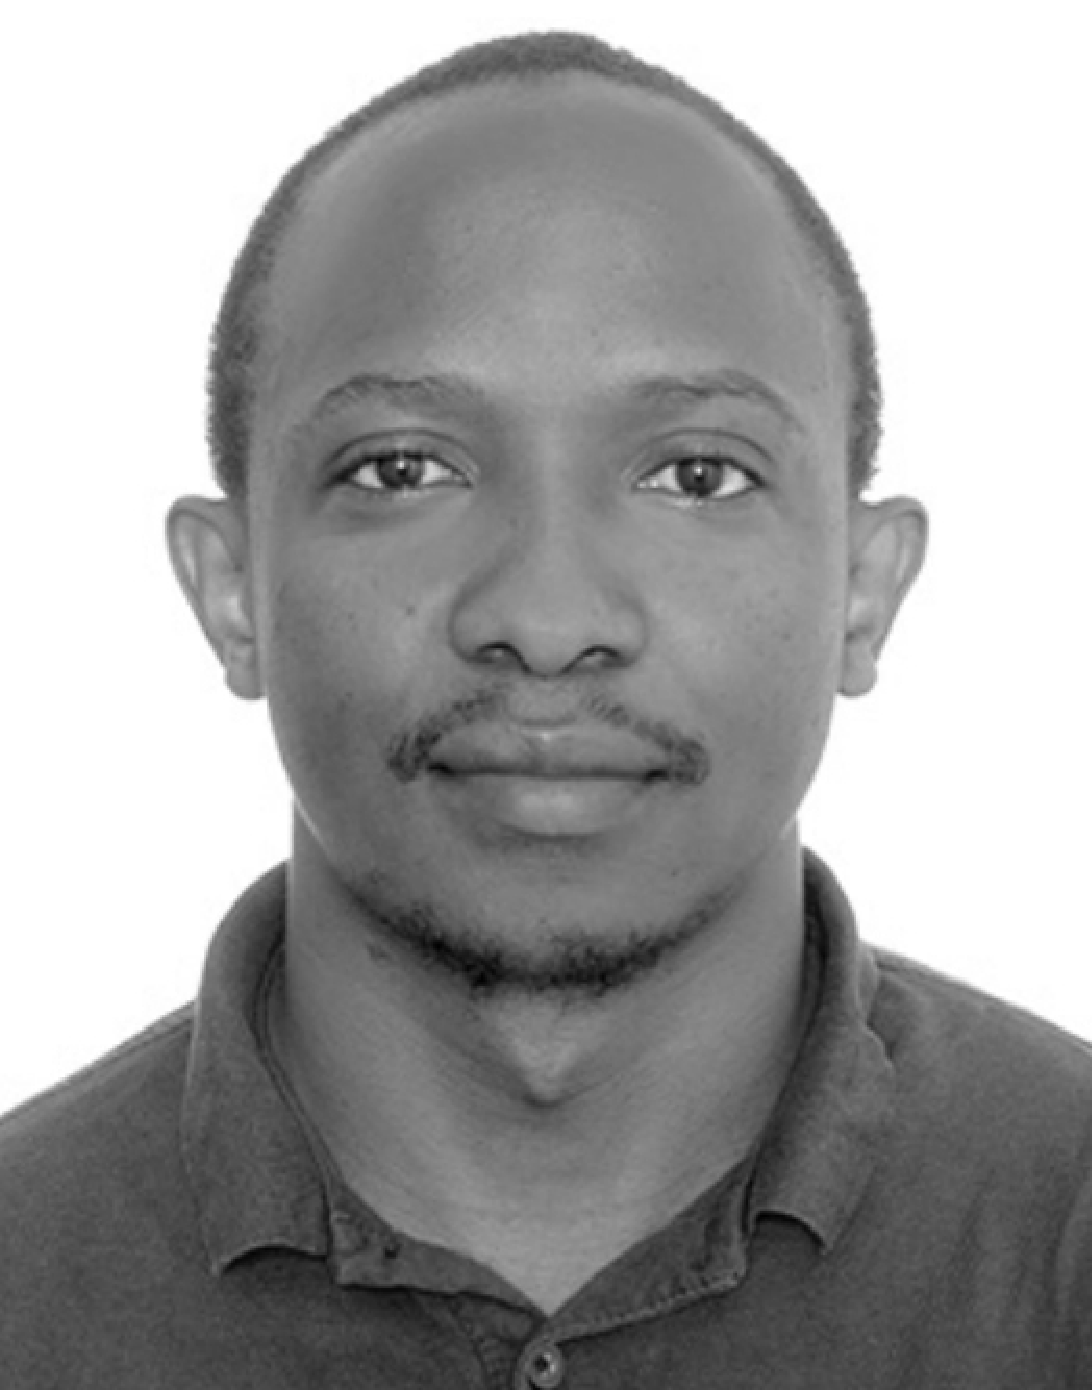
\includegraphics[width=1in,height=1.25in,clip,keepaspectratio]{format/author2.pdf}}]
{Dr. Godfrey M. Kibalya}~received his B.Sc. degree in telecommunications engineering from Makerere University, Uganda, in 2010, his M.Sc. degree in telecommunications engineering from the University of Trento, Italy, and his Ph.D. degree in network engineering from the Technical University of Catalonia (UPC), Spain. He is a Senior Researcher at Nearby Computing S.L. His previous experience includes work in telecommunications engineering in Uganda. Dr. Kibalya's research interests focus on network function virtualization and the application of artificial intelligence in network management. He is actively involved in advancing the field of telecommunications through his research and teaching roles.
\end{IEEEbiography}%

\begin{IEEEbiography}
[{
\includegraphics[width=1in,height=1.25in,clip,keepaspectratio]{format/author3.pdf}}]
{Dr. Angelos Antonopoulos}~(Senior Member, IEEE) is currently the Research and Innovation Director
at Nearby Computing S.L. He has authored over 130 papers on various topics, including multi-access edge computing, 5G/6G network architectures, network virtualization/slicing, 5G-ready vertical and over-the-top applications, zero-touch service orchestration, and analytical modeling/optimization in mobile networks.
He has received the Best Paper Award at IEEE GLOBECOM 2014, the Best Demo Award at IEEE CAMAD 2014, and the EURACON Best Paper Award at EuCNC 2016. He has been awarded with the First Prize in the IEEE ComSoc Student Competition (as a Mentor), while he was the Director of the Best UPC Thesis in ICT (2018). He has been on the editorial board of the IEEE Access, IEEE Networking Letters, Computer Networks (Elsevier), and Inventions (MDPI). He has served as officer (Secretary and Vice-Chair) of the IEEE ComSoc Technical Committee on Communication Systems Integration and Modeling (CSIM) and he is an IEEE Senior Member.
\end{IEEEbiography}

\vfill\pagebreak

% Debug information
% End of document reached

% Debug information
% End of document reached
\end{document}
